\chapter{Spettro, Multiplexing e Modulazione Digitale}
Nel capitolo precedente abbiamo studiato come un'onda radio si propaga nello spazio. Ora affrontiamo due domande complementari: \emph{come si dividono le risorse} di un mezzo condiviso (lo spettro) tra più utenti, e \emph{come si codificano i bit} su un'onda radio (la modulazione). Sono questi i meccanismi che trasformano un canale fisico rumoroso in un canale logico capace di trasportare informazione.

\section{Lo Spettro Elettromagnetico}
Le onde radio occupano una porzione dello spettro elettromagnetico che va, grossolanamente, da poche decine di kHz fino a centinaia di GHz, al di sotto delle frequenze dell'infrarosso e della luce visibile. Ogni tecnologia wireless opera in una specifica \textbf{banda di frequenza}.

\dfn{Banda licenziata e non licenziata}{
    Lo spettro è una risorsa scarsa e regolamentata da enti governativi. Una banda \textbf{licenziata} (es. GSM, UMTS) è assegnata in esclusiva a un operatore, che paga per l'uso e ne ha protezione legale dalle interferenze. Una banda \textbf{non licenziata} (es. la banda \textbf{ISM} a 2.4 GHz usata da Wi-Fi, Bluetooth, ZigBee) è di libero utilizzo nel rispetto di limiti di potenza, ma non offre alcuna garanzia contro le interferenze altrui.
}

\subsection{Larghezza di banda e capacità}
Una domanda naturale è: perché canali diversi possono avere capacità (bit/s) diverse? Non è perché i bit "viaggiano più veloci" — tutti i segnali si propagano alla velocità della luce. La differenza sta nella \textbf{larghezza di banda} (bandwidth) assegnata al canale: una banda più larga permette di accomodare (codificare) un bit sul canale in meno tempo, e quindi di trasmettere più bit al secondo.

\nt{La capacità di un canale cresce con la larghezza di banda disponibile e con la qualità del segnale (rapporto segnale/rumore). È questo il legame, formalizzato dal teorema di Shannon, tra risorse fisiche e velocità raggiungibile.}

\subsection{Classificazione per copertura}
Le reti wireless si classificano in base all'estensione geografica coperta:
\begin{itemize}
    \item \textbf{WWAN} (Wide Area Network): copertura geografica, es. reti cellulari e satellitari.
    \item \textbf{WMAN} (Metropolitan Area Network): copertura metropolitana, es. WiMAX.
    \item \textbf{WLAN} (Local Area Network): copertura locale, es. Wi-Fi (campus, edificio, casa).
    \item \textbf{WPAN} (Personal Area Network): copertura ridotta attorno alla persona, es. Bluetooth, ZigBee.
\end{itemize}
In generale, all'aumentare della copertura diminuisce il data rate per utente e aumenta il supporto alla mobilità.

\subsection{Modalità di rete: Ad-Hoc e Infrastructure}
\begin{itemize}
    \item \textbf{Infrastructure}: esiste un'unità di controllo centralizzata (\textbf{Access Point} o stazione base) a cui i terminali mobili si associano. L'AP gestisce la condivisione delle risorse, il \textit{roaming} tra celle e la connessione al backbone cablato.
    \item \textbf{Ad-Hoc}: comunicazione \textit{peer-to-peer} "al volo", senza infrastruttura preesistente. La rete \emph{è} l'insieme dei dispositivi stessi: nessuna amministrazione né configurazione.
\end{itemize}

\section{Multiplexing: condividere il mezzo}
Il multiplexing è l'insieme delle tecniche che permettono a più comunicazioni di condividere lo stesso mezzo trasmissivo. Si può operare lungo \textbf{quattro dimensioni}: spazio, tempo, frequenza e codice.

\begin{center}
    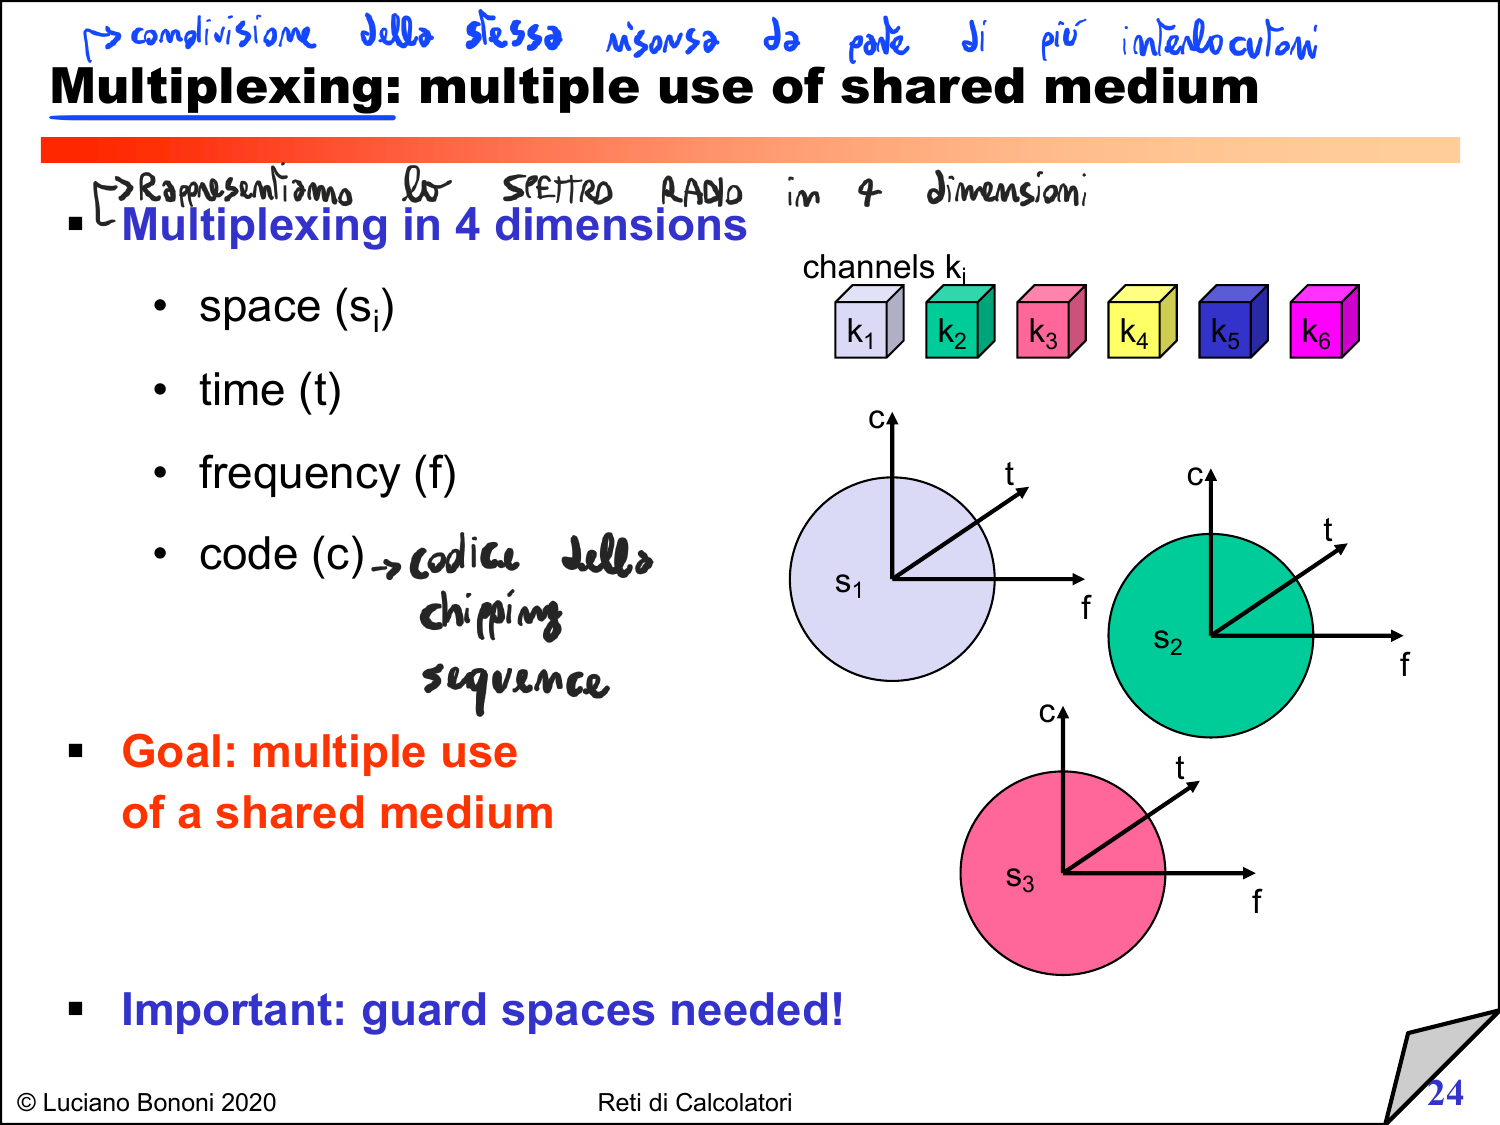
\includegraphics[width=12cm]{img/multiplexing_4d.png}
\end{center}

\nt{In tutte le tecniche di multiplexing sono necessari degli \textbf{spazi di guardia} (guard spaces): intervalli di separazione (in tempo, frequenza, ecc.) per evitare che canali adiacenti interferiscano tra loro.}

\subsection{Frequency Division Multiplexing (FDM)}
Lo spettro viene suddiviso in bande di frequenza più piccole; ogni canale riceve una banda per tutto il tempo.
\begin{itemize}
    \item \textbf{Vantaggi}: nessun coordinamento dinamico necessario; funziona anche con segnali analogici.
    \item \textbf{Svantaggi}: spreco di banda se il traffico è distribuito in modo non uniforme; inflessibile; richiede spazi di guardia in frequenza.
\end{itemize}

\subsection{Time Division Multiplexing (TDM)}
Ogni canale ottiene tutto lo spettro, ma solo per un certo intervallo di tempo (slot).
\begin{itemize}
    \item \textbf{Vantaggi}: una sola portante nel mezzo in ogni istante; throughput elevato anche con molti utenti.
    \item \textbf{Svantaggi}: richiede una sincronizzazione precisa tra le stazioni.
\end{itemize}

\subsection{TDM + FDM combinati}
Un canale ottiene una certa banda di frequenza per un certo intervallo di tempo. È lo schema usato dal \textbf{GSM}. Offre migliore protezione dalle intercettazioni e dalle interferenze selettive in frequenza, e data rate più alti rispetto al solo code multiplex, ma richiede un coordinamento preciso.

\subsection{Code Division Multiplexing (CDM)}
Ogni canale è identificato da un \textbf{codice} univoco; tutti i canali usano lo stesso spettro nello stesso istante.
\begin{itemize}
    \item \textbf{Vantaggi}: efficiente in banda; nessun coordinamento né sincronizzazione tra canali; buona protezione da interferenze e intercettazioni.
    \item \textbf{Svantaggi}: data rate per utente più bassi; rigenerazione del segnale più complessa (costosa).
\end{itemize}
È implementato tramite tecnologia \textit{spread spectrum} (vedi più avanti, CDMA).

\subsection{Riuso delle frequenze (Frequency Reuse)}
Nelle reti cellulari la stessa frequenza può essere riutilizzata in celle sufficientemente distanti, in modo che le interferenze siano trascurabili. Il modello classico usa un \textbf{cluster di 7 frequenze}.
\begin{itemize}
    \item \textbf{Assegnazione fissa}: frequenze prestabilite per ogni cella. Problema: carico di traffico diverso nelle varie celle.
    \item \textbf{Assegnazione dinamica}: la stazione base sceglie le frequenze in base a quelle già usate nelle celle vicine (o a misure di interferenza), dando più capacità alle celle più cariche.
\end{itemize}

\section{La Modulazione}
\dfn{Modulazione}{
    Il processo di codifica dell'informazione (i bit) variando uno o più parametri di un'onda portante (carrier) ad alta frequenza. La modulazione \textbf{digitale} traduce dati digitali in un segnale analogico in banda base; la modulazione \textbf{analogica} sposta poi questo segnale sulla frequenza della portante radio.
}

\paragraph{Perché modulare?} Le motivazioni sono tre:
\begin{itemize}
    \item \textbf{Antenne più piccole}: l'antenna efficiente ha dimensioni dell'ordine di $\lambda/4$; salire in frequenza riduce $\lambda$ e quindi la dimensione dell'antenna.
    \item \textbf{Multiplexing in frequenza}: spostare comunicazioni diverse su portanti diverse (FDM).
    \item \textbf{Caratteristiche del mezzo}: certe frequenze si propagano meglio in certi ambienti.
\end{itemize}

Gli schemi di base modulano uno dei tre parametri dell'onda: ampiezza (AM), frequenza (FM) o fase (PM).

\subsection{Tecniche di modulazione digitale (Shift Keying)}
\begin{center}
    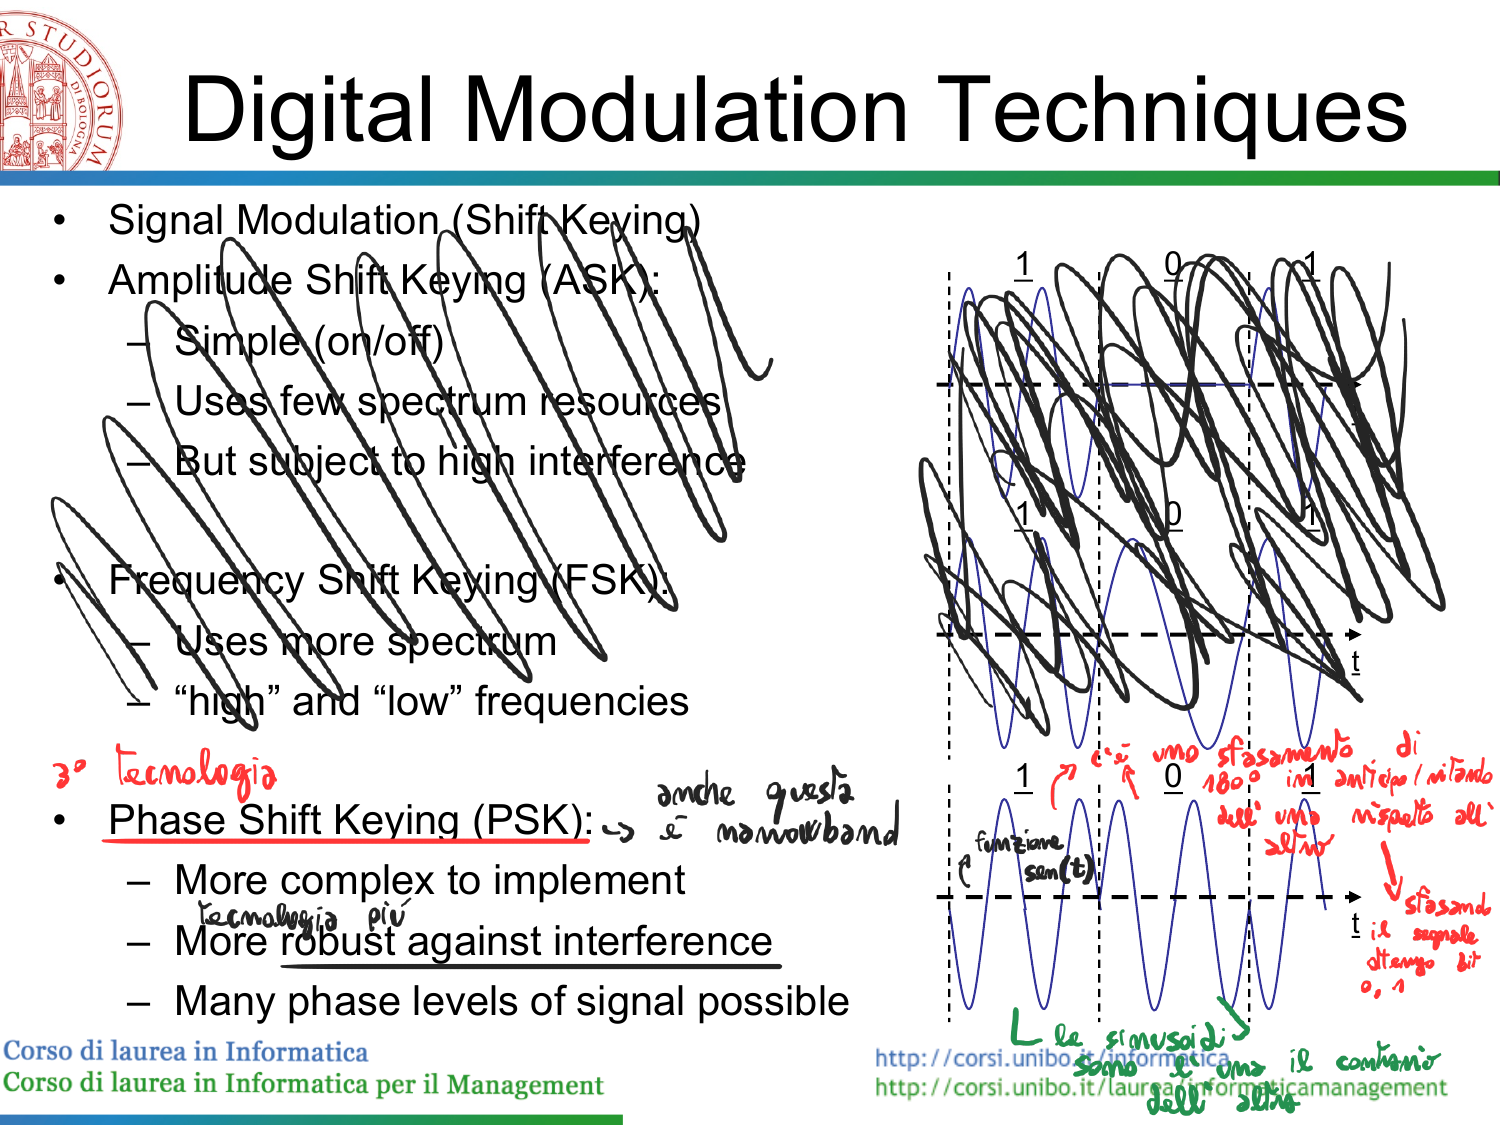
\includegraphics[width=10cm]{img/modulazione_ask_fsk_psk.png}
\end{center}
\begin{itemize}
    \item \textbf{ASK (Amplitude Shift Keying)}: il bit è codificato dall'ampiezza (es. on/off). Semplice e parco di spettro, ma molto sensibile alle interferenze (che agiscono proprio sull'ampiezza).
    \item \textbf{FSK (Frequency Shift Keying)}: si usano due frequenze diverse per "0" e "1". Usa più spettro, ma è più robusto dell'ASK.
    \item \textbf{PSK (Phase Shift Keying)}: l'informazione è nella fase del segnale. Più complesso da implementare, ma robusto contro le interferenze e capace di molti livelli di fase.
\end{itemize}

\subsection{Rappresentazione del segnale e simboli}
Un segnale radio può essere rappresentato in tre domini: (a) \textbf{ampiezza} nel tempo; (b) \textbf{frequenza}; (c) \textbf{diagramma di costellazione}, in cui ogni punto rappresenta uno stato (ampiezza $M$ e fase $\varphi$) in coordinate polari, scomposto nelle componenti $I = M\cos\varphi$ (in-phase) e $Q = M\sin\varphi$ (quadrature).

\dfn{Simbolo}{
    Uno stato (combinazione di ampiezza e fase) che la portante assume durante la trasmissione. Ogni simbolo trasporta uno o più bit; la sequenza di bit viene trasmessa facendo assumere all'onda, in successione, le caratteristiche dei simboli associati.
}

\paragraph{BPSK e QPSK.}
\begin{itemize}
    \item \textbf{BPSK} (Binary PSK): due simboli sfasati di $180\dg$ (es. bit 0 in fase $0\dg$, bit 1 in fase $180\dg$). 1 bit per simbolo. Semplice e robusto (usato nelle comunicazioni satellitari), ma a bassa efficienza spettrale.
    \item \textbf{QPSK} (Quadrature PSK): quattro simboli sfasati di $90\dg$, ciascuno codifica \textbf{2 bit}. Raddoppia il bit rate a parità di simboli al secondo, ma è più vulnerabile: i simboli sono più "vicini" tra loro nella costellazione.
\end{itemize}

\begin{center}
    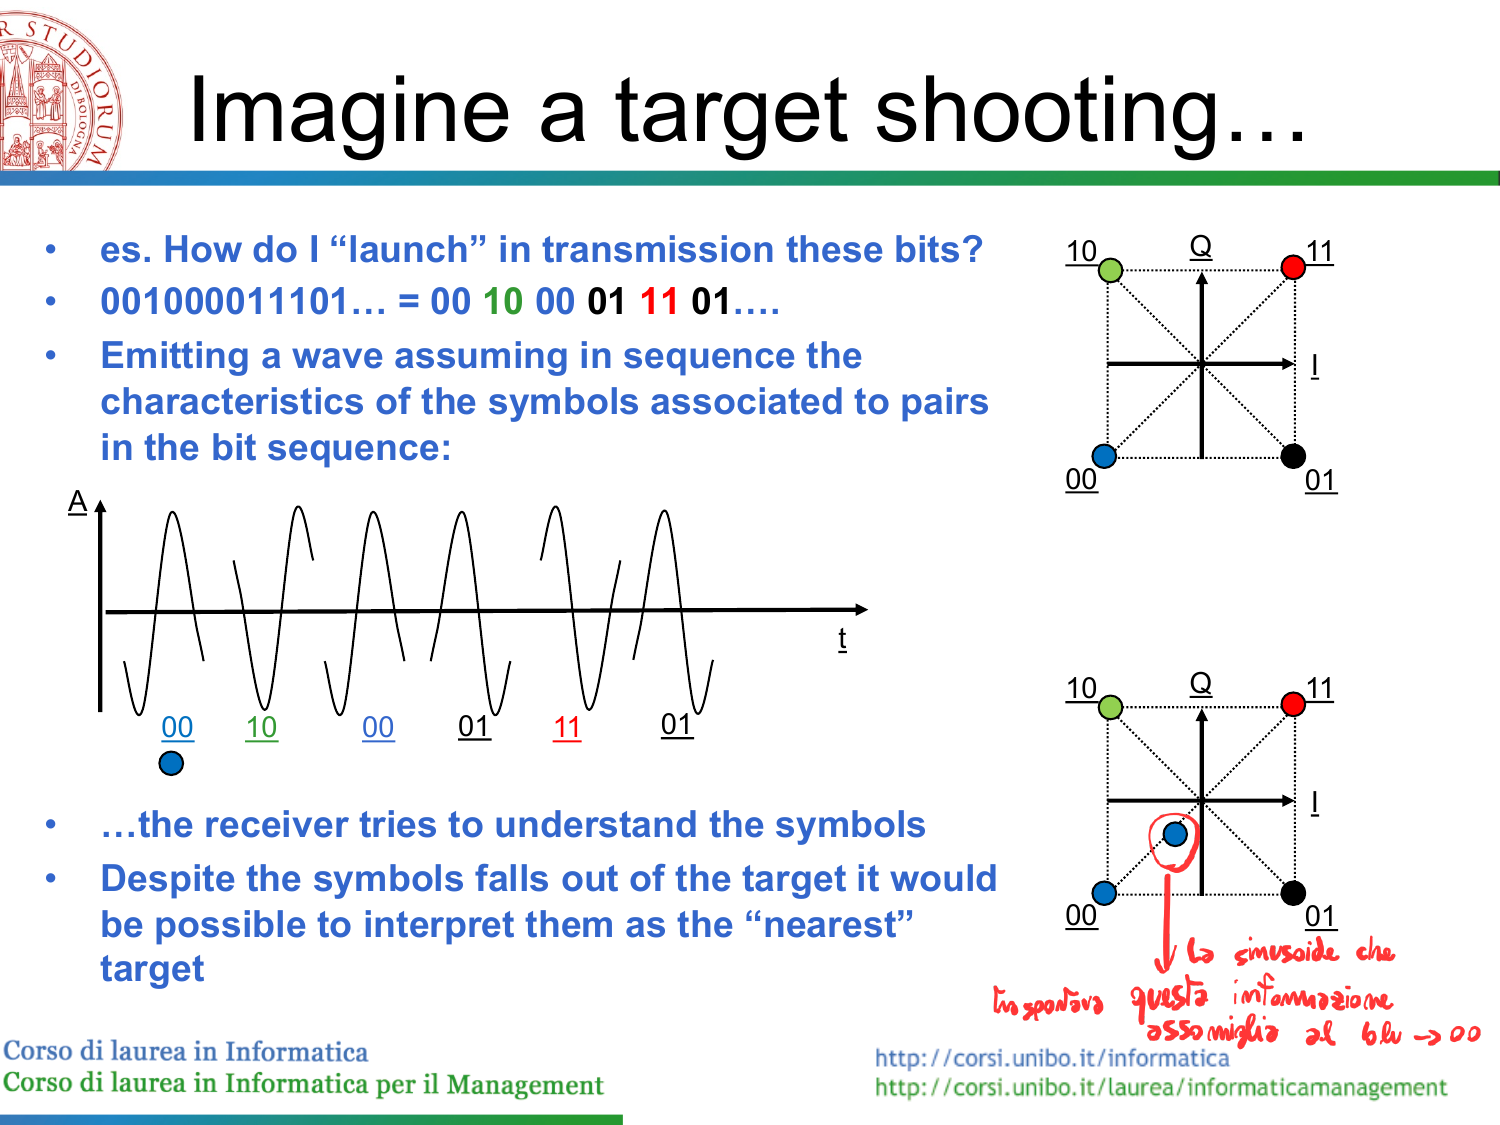
\includegraphics[width=8cm]{img/costellazione_qpsk.png}
\end{center}

\subsection{L'analogia del "tiro al bersaglio"}
Si può pensare alla ricezione come a un tiro al bersaglio: ogni simbolo trasmesso "atterra" in un punto della costellazione e il ricevitore lo interpreta come il simbolo (bersaglio) più vicino. Il rumore sposta il punto ricevuto.

\qs{Quando si verifica un errore?}{
    Quando il rumore sposta il simbolo ricevuto talmente tanto da uscire dall'area del proprio bersaglio, finendo nell'area di un simbolo adiacente: il ricevitore decodifica i bit sbagliati.
}

Da qui due osservazioni fondamentali sul \emph{compromesso} efficienza/robustezza:
\begin{enumerate}
    \item Più simboli (costellazione densa) $\Rightarrow$ più bit per simbolo $\Rightarrow$ aree del bersaglio più piccole $\Rightarrow$ più sensibilità al rumore. Quando il canale è rumoroso conviene scendere a una costellazione rada (es. BPSK, area grande, tutti i bit corretti ma metà del bit rate); quando il canale è buono si può "spingere sull'acceleratore" usando costellazioni dense.
    \item Un simbolo errato finisce con alta probabilità in un bersaglio \emph{adiacente}. Conviene quindi etichettare i simboli con un \textbf{codice di Gray}, in cui simboli adiacenti differiscono per \emph{un solo bit}: così un errore di simbolo causa un solo bit errato anziché due o più.
\end{enumerate}

\nt{Il legame con il \textbf{rilevamento d'errore}: se al massimo 1 bit è errato, un semplice \textbf{bit di parità} permette di rilevarlo; organizzando i bit in una \textbf{matrice con parità di riga e di colonna} si può perfino localizzare e correggere il singolo bit errato (come nel gioco della battaglia navale). Per questo è importante minimizzare il numero di bit che cambiano tra simboli adiacenti.}

\subsection{Quadrature Amplitude Modulation (QAM)}
\dfn{QAM}{
    Tecnica che combina la modulazione di \emph{ampiezza e fase} dello stesso simbolo. Con $2^n$ simboli definiti, ogni simbolo codifica $n$ bit. Aumentando $n$ cresce il bit rate, ma l'area di ciascun bersaglio si riduce e cresce la sensibilità al rumore.
}

\begin{center}
    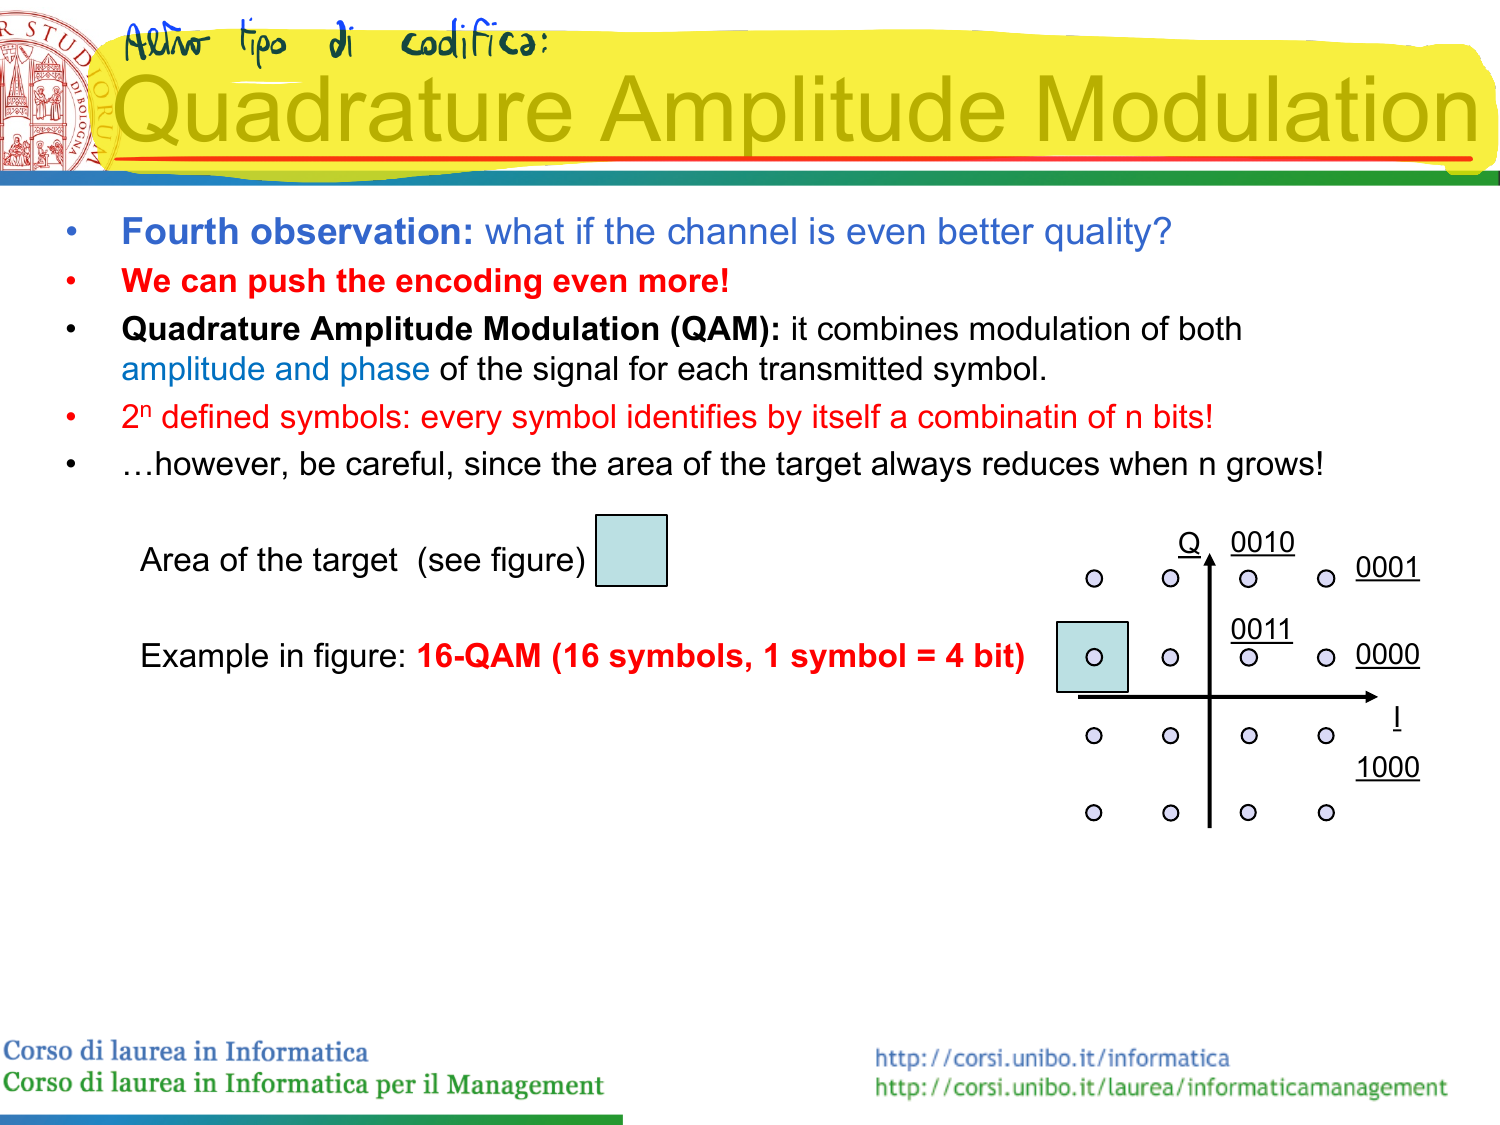
\includegraphics[width=7cm]{img/qam16.png}
\end{center}

Esempio: il \textbf{16-QAM} usa 16 simboli (1 simbolo = 4 bit); simboli con la stessa fase ma ampiezza diversa sono distinti. È usato in modem, TV digitale e WiMAX. Wi-Fi moderno arriva fino a 256-QAM e oltre.

\subsection{Modulazione Gerarchica (Hierarchical Modulation)}
\dfn{Modulazione Gerarchica}{
    Schema che modula \emph{due} flussi di bit con priorità diverse nello stesso simbolo. Nel 64-QAM gerarchico, i 6 bit di ogni simbolo si dividono in 2 bit ad \textbf{alta priorità} (la "nuvola" — gruppo di simboli — in cui cade il punto) e 4 bit a \textbf{bassa priorità} (la posizione esatta dentro la nuvola).
}

\begin{center}
    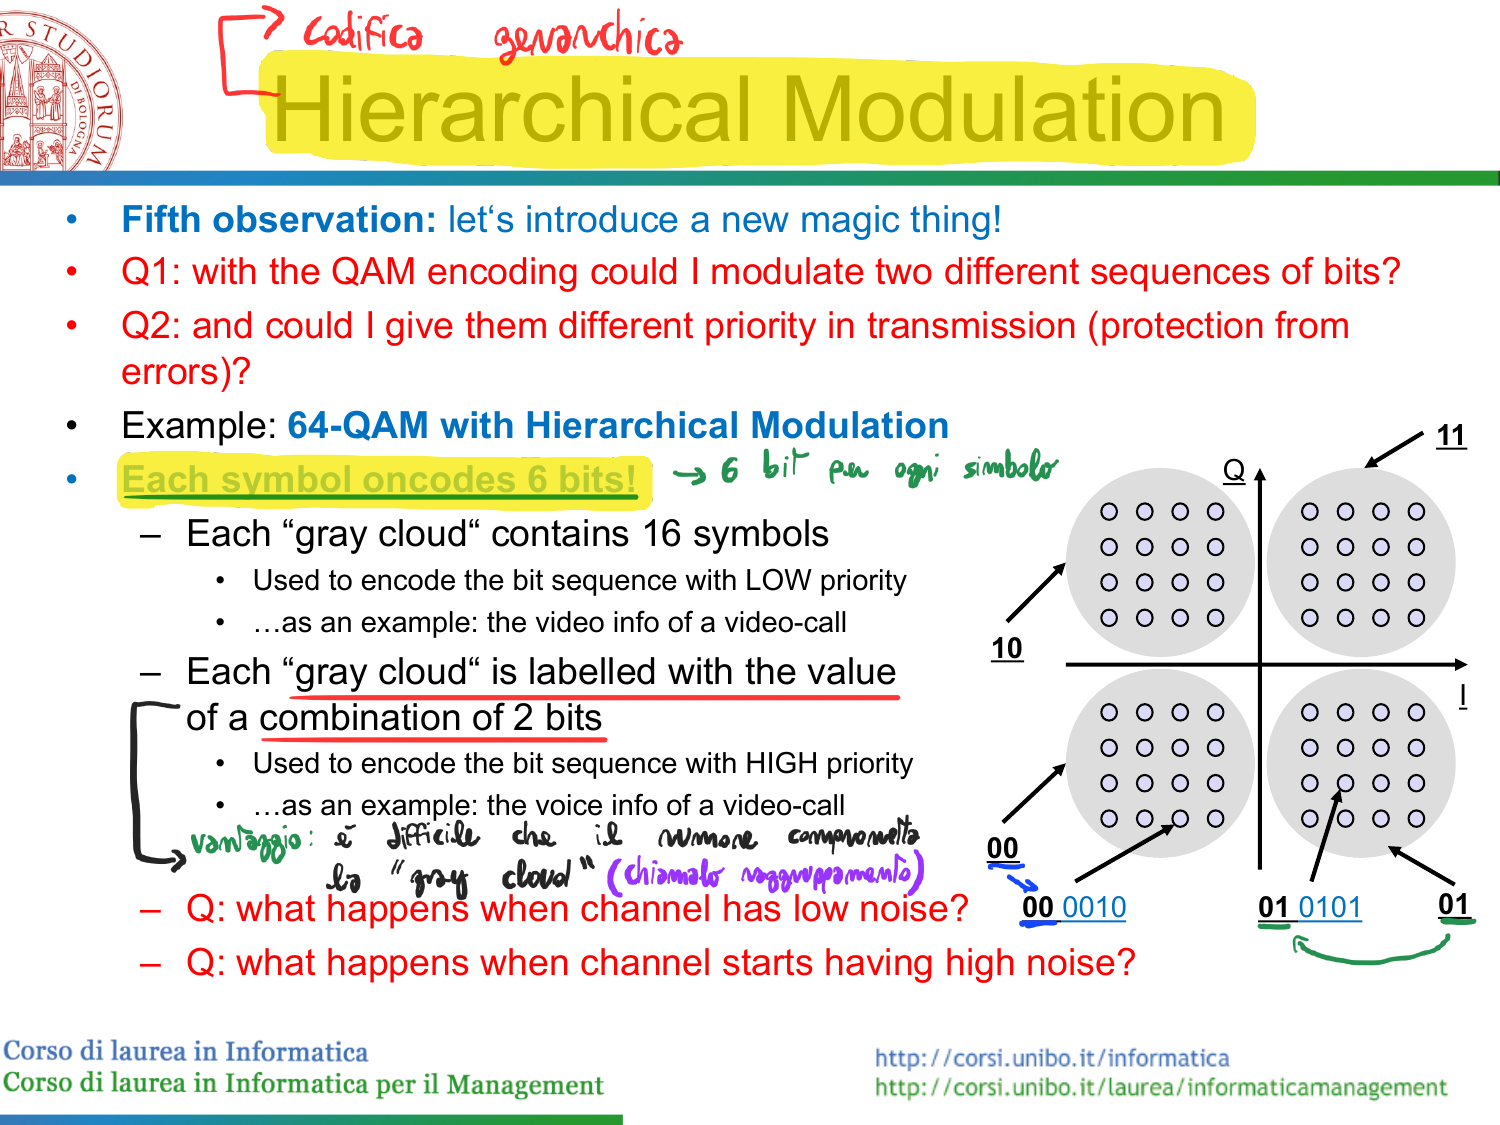
\includegraphics[width=7cm]{img/hierarchical_modulation.png}
\end{center}

\ex{Video-chiamata mobile}{
    In una video-chiamata, la \textbf{voce} (più importante) viene codificata nei 2 bit ad alta priorità e il \textbf{video} nei 4 bit a bassa priorità. Con canale a basso rumore tutti i simboli sono colpiti correttamente: voce e video arrivano integri. Quando il rumore aumenta, i singoli simboli dentro una nuvola diventano indistinguibili (video corrotto), ma la nuvola corretta è quasi sempre individuata: il ricevitore recupera comunque la voce \emph{sacrificando} la qualità del video. È un esempio di degradazione "graziosa" della qualità.
}

\section{Spread Spectrum}
\dfn{Spread Spectrum}{
    Tecnica che "spalma" un segnale a banda stretta (narrowband) su una banda molto più larga (broadband), usando un codice. A un ricevitore non intenzionale il segnale appare come rumore di fondo a bassa potenza.
}

\paragraph{Motivazione.} Un'interferenza dipendente dalla frequenza (\textit{frequency selective fading}) può cancellare completamente un segnale a banda stretta per tutta la durata del disturbo. Spalmando il segnale su una banda larga, solo una piccola frazione viene colpita e l'informazione si recupera. Effetti collaterali positivi: coesistenza di più segnali senza coordinamento dinamico, e \emph{tap-proof} (non decodificabile senza conoscere il codice).

\nt{Intuizione: trasmettere "Hello World" su un'unica frequenza (narrowband) significa che un disturbo su quella frequenza distrugge interi caratteri. Trasmetterlo "spalmato" su molte frequenze (broadband) fa sì che il disturbo ne colpisca solo qualche pezzetto, recuperabile.}

\subsection{Direct Sequence Spread Spectrum (DSSS)}
\dfn{DSSS}{
    Ogni bit dei dati viene messo in XOR con una sequenza pseudo-casuale di \textbf{chip} (chipping sequence o sequenza di Barker). Avere molti chip per bit (es. 128) allarga la banda del segnale. Sequenze lunghe aumentano la probabilità di recuperare il bit originale anche senza ritrasmissione.
}

\begin{center}
    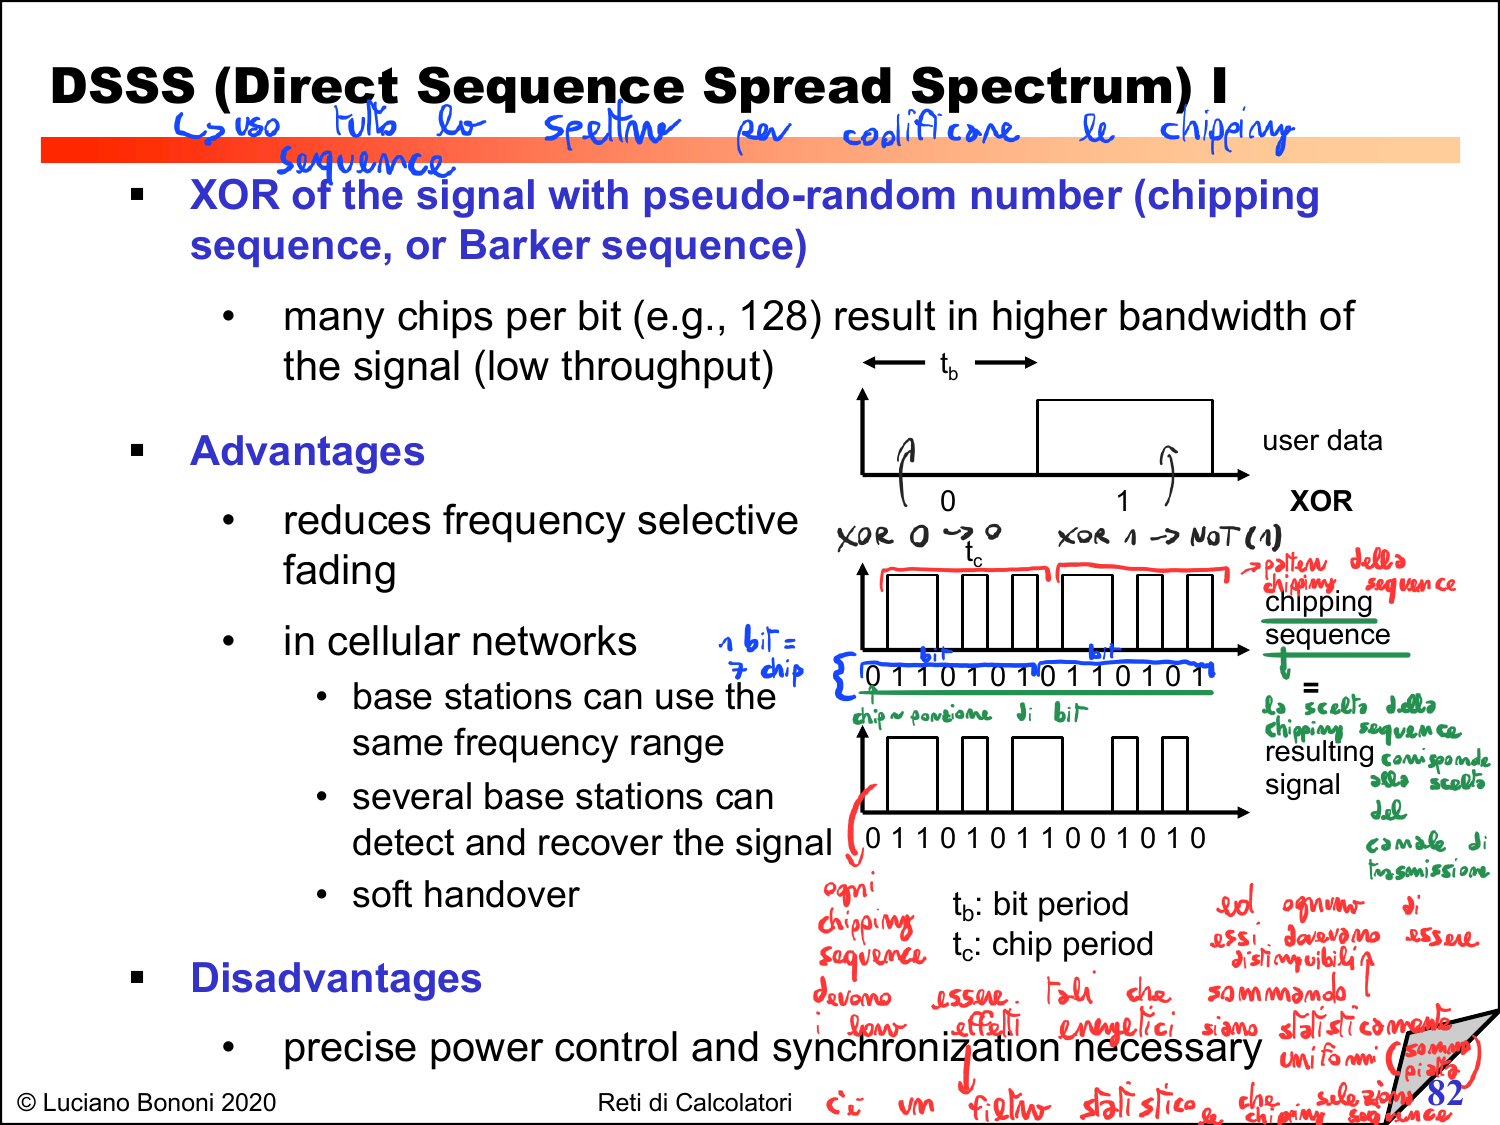
\includegraphics[width=9cm]{img/dsss_xor.png}
\end{center}

\begin{itemize}
    \item \textbf{Vantaggi}: riduce il frequency selective fading; nelle reti cellulari più stazioni base possono usare la stessa banda e rilevare il segnale (consente il \textit{soft handover}).
    \item \textbf{Svantaggi}: richiede controllo di potenza e sincronizzazione precisi.
\end{itemize}

\paragraph{Canali 802.11b.} Lo standard 802.11b (DSSS) nella banda 2.4 GHz definisce 14 canali spaziati di 5 MHz, ma ogni canale occupa $\sim$22 MHz. Per evitare sovrapposizioni servono $\sim$25 MHz di spaziatura: i tre canali \textbf{1, 6, 11} sono gli unici reciprocamente \textbf{non sovrapposti} e per questo usati per il riuso in WLAN adiacenti.

\subsection{Code Division Multiple Access (CDMA)}
Il CDMA è l'applicazione del code multiplexing tramite spread spectrum: ogni mittente ha una \textbf{chiave} (codice) ortogonale e tutti trasmettono contemporaneamente sulla stessa banda. Il ricevitore isola il mittente desiderato applicando la sua chiave.

\ex{CDMA: esempio numerico}{
    Convenzione: bit "0"$\,=-1$, bit "1"$\,=+1$. Le chiavi sono sequenze di $\pm1$.
    \begin{itemize}
        \item \textbf{Mittente A}: dato $A_d = 1$, chiave $A_k = (-1,+1,-1,-1,+1,+1)$. Segnale inviato $A_s = A_d \cdot A_k = (-1,+1,-1,-1,+1,+1)$.
        \item \textbf{Mittente B}: dato $B_d = 0$, chiave $B_k = (+1,+1,-1,+1,-1,+1)$. Segnale inviato $B_s = B_d \cdot B_k = (-1,-1,+1,-1,+1,-1)$.
        \item I segnali si sovrappongono nello spazio: $A_s + B_s = (-2,0,0,-2,+2,0)$.
    \end{itemize}
    Il ricevitore che vuole \textbf{A} calcola il prodotto interno con $A_k$:
    $$ (A_s+B_s)\cdot A_k = 2+0+0+2+2+0 = 6 > 0 \;\Rightarrow\; \text{bit } 1. $$
    Per ricevere \textbf{B} usa $B_k$:
    $$ (A_s+B_s)\cdot B_k = -2+0+0-2-2+0 = -6 < 0 \;\Rightarrow\; \text{bit } 0. $$
    Una chiave \emph{sbagliata} dà invece un risultato vicino a zero (nessun bit riconoscibile). Chiavi reali, molto più lunghe, garantiscono grande distanza tra le parole di codice.
}

\begin{center}
    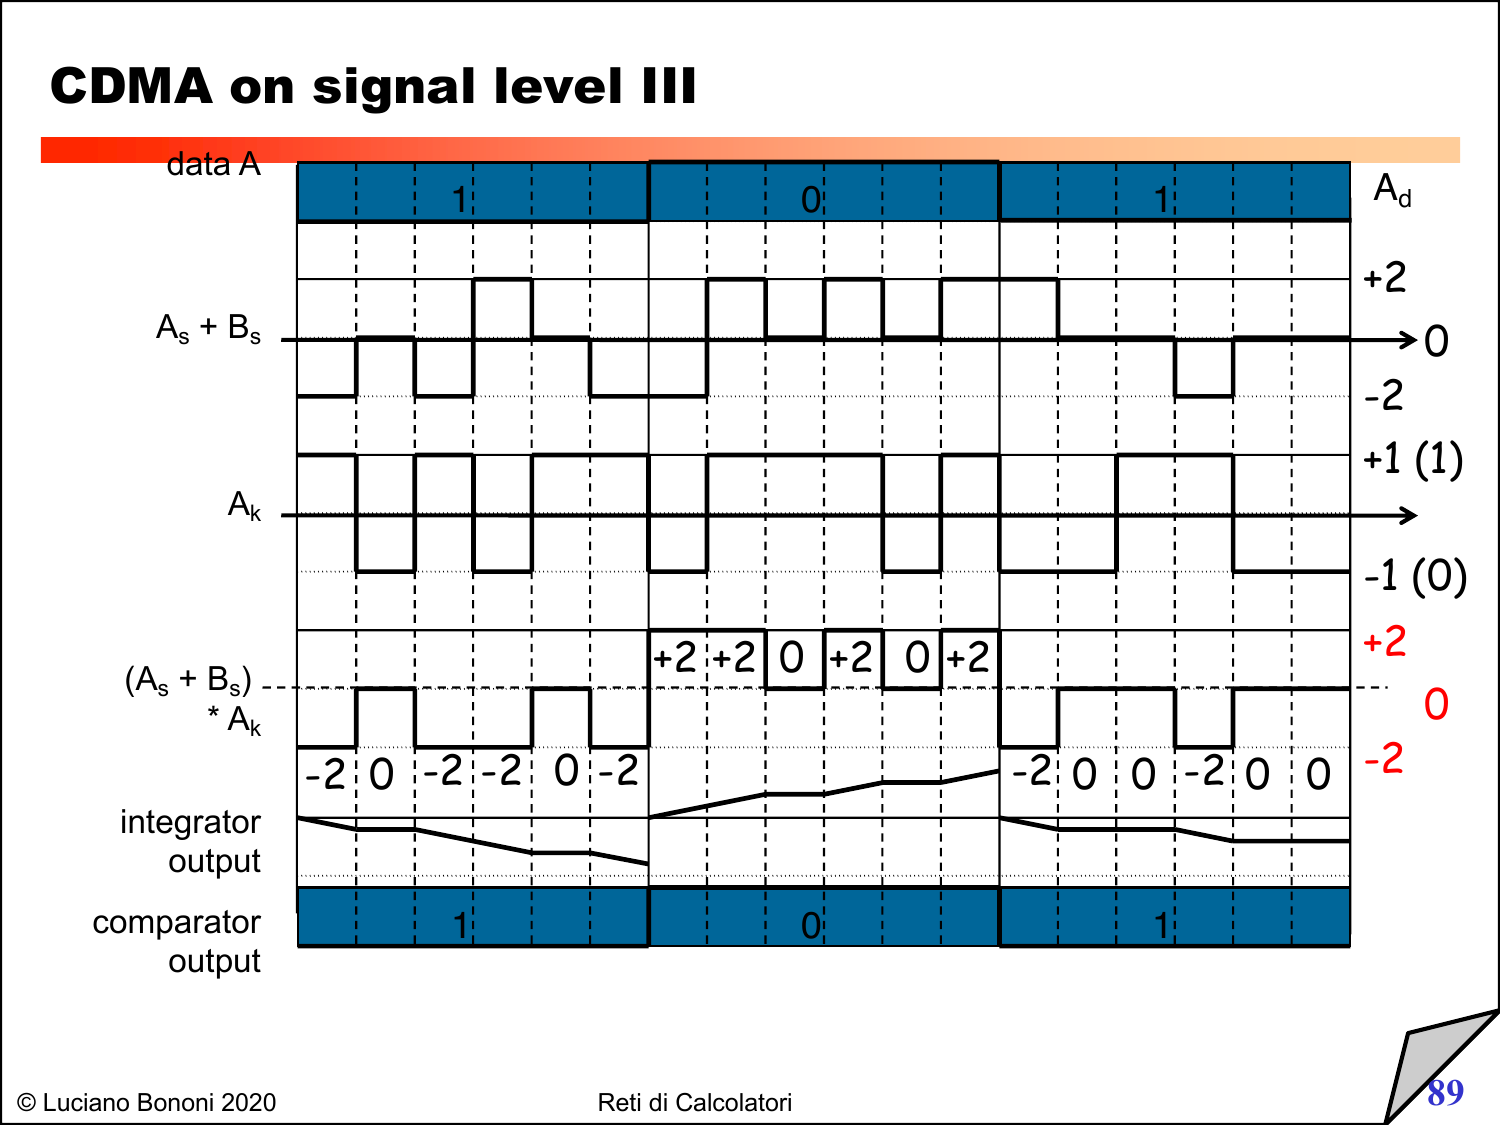
\includegraphics[width=9cm]{img/cdma_signal_level.png}
\end{center}

\subsection{Frequency Hopping Spread Spectrum (FHSS)}
\dfn{FHSS}{
    La portante a banda stretta cambia frequenza nel tempo seguendo una sequenza di "salti" (hopping) pseudo-casuale nota a mittente e ricevitore. A un ricevitore non intenzionale appare come rumore impulsivo. La sequenza di salti è generata da un seed (es. in Bluetooth dipende dall'identificativo del dispositivo).
}

\begin{center}
    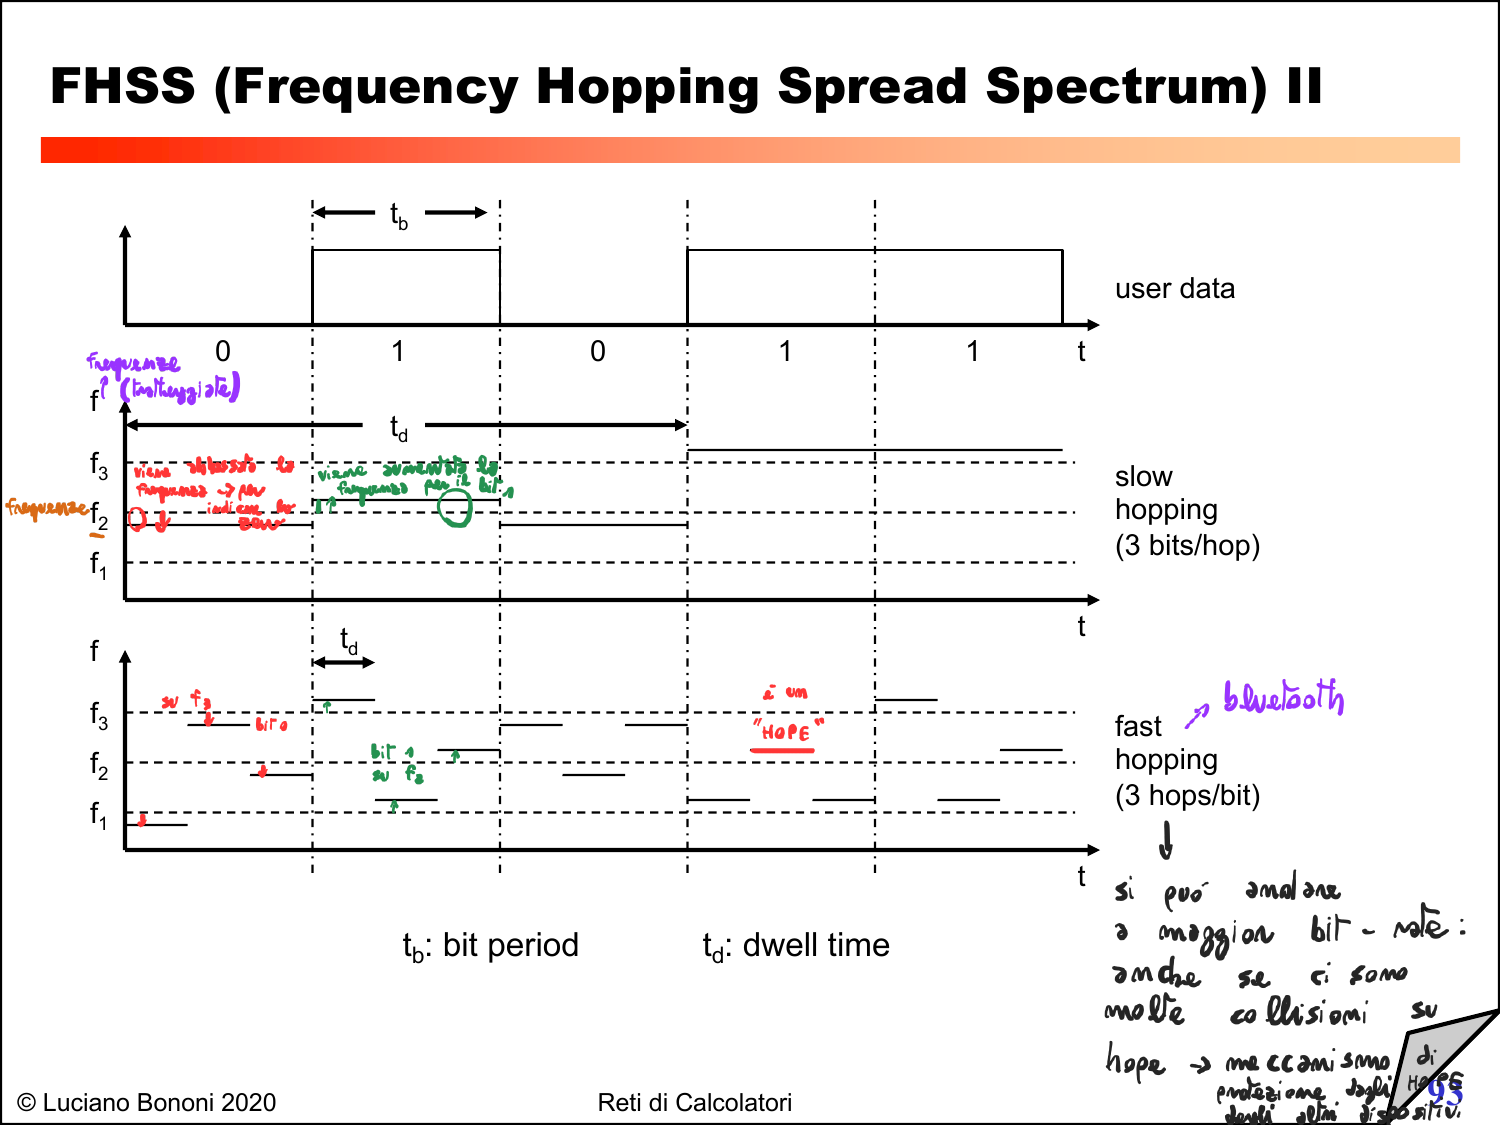
\includegraphics[width=9cm]{img/fhss_hopping.png}
\end{center}

Due varianti: \textbf{slow hopping} (più bit per salto) e \textbf{fast hopping} (più salti per bit). Vantaggi: fading e interferenze selettive limitati a brevi periodi; implementazione semplice; usa solo una piccola porzione di spettro per volta. Svantaggi: meno robusto del DSSS e più facile da rilevare.

\section{OFDM (Orthogonal Frequency Division Multiplexing)}
\dfn{OFDM}{
    Evoluzione dell'FDM in cui un singolo canale è suddiviso in molte \textbf{sotto-portanti} (subcarrier) su frequenze adiacenti \emph{sovrapposte} ma \textbf{ortogonali}. L'ortogonalità (l'integrale del prodotto di due sotto-portanti su un periodo è nullo) consente trasmissioni simultanee senza interferenza reciproca e \emph{senza spazi di guardia}, con alta efficienza spettrale.
}

\begin{center}
    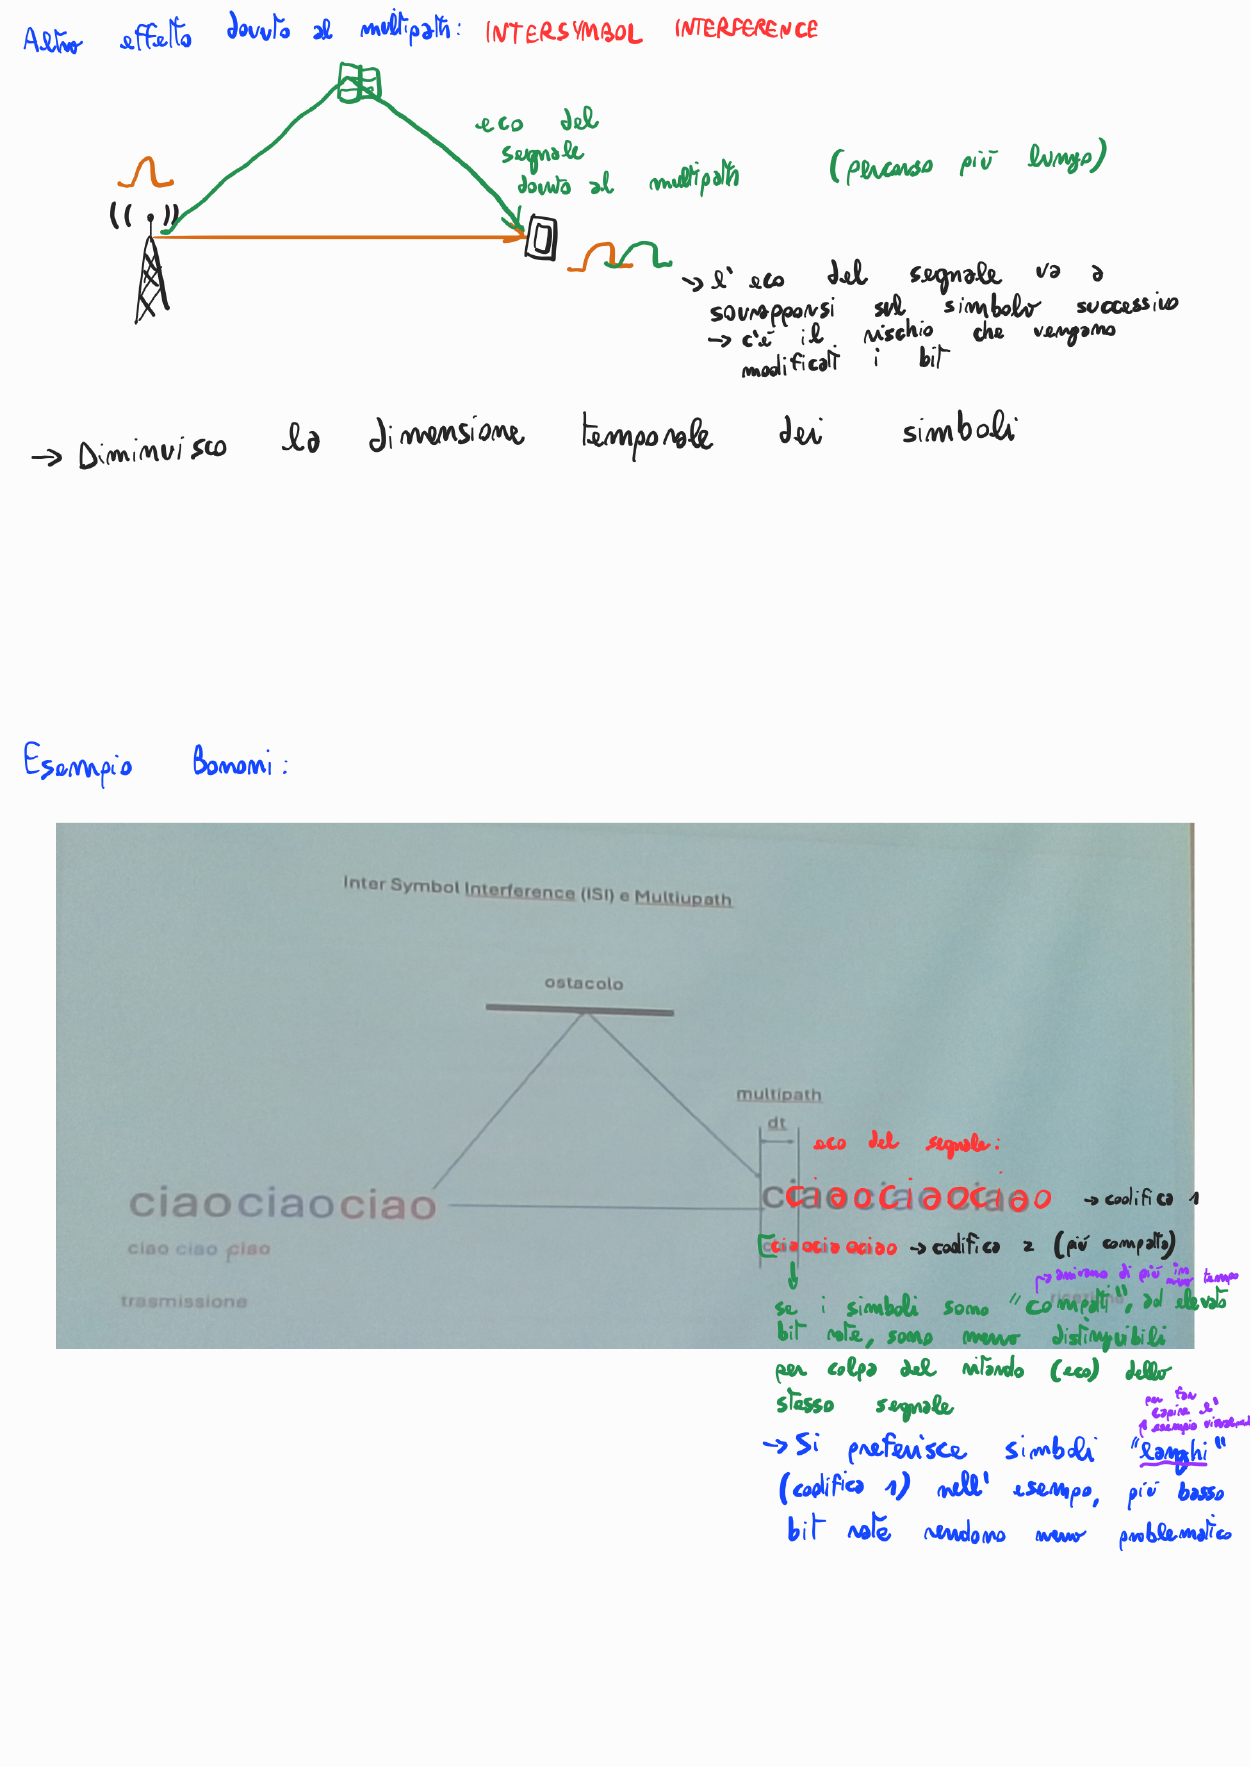
\includegraphics[width=10cm]{img/ofdm_vs_fdm.png}
\end{center}

\begin{itemize}
    \item I dati sono trasmessi in parallelo su molte sotto-portanti; non serve un filtro separato per ogni sotto-canale (come invece in FDM).
    \item Implementato efficientemente con chip a basso costo per la \textbf{Trasformata di Fourier Veloce (FFT/IFFT)}: i bit sono visti come ampiezze di frequenze e la IFFT li trasforma in segnale nel tempo (e viceversa in ricezione).
    \item Esempio 802.11g/a: canale da 20 MHz suddiviso in 52 sotto-portanti ($\sim$300 kHz), di cui 48 per i dati e 4 come piloti di gestione. Usa convolutional coding per la correzione d'errore.
    \item Usato in 802.11a/g/n/ac, WiMAX (802.16) e LTE. Problema: a velocità elevate lo \textit{shift Doppler} sposta le frequenze delle sotto-portanti.
\end{itemize}

\nt{L'OFDM dell'802.11g \textbf{non} è compatibile con il DSSS dell'802.11b: pur condividendo la banda 2.4 GHz, usano schemi di modulazione diversi.}

\section{Conclusione}
A parità di condizioni fisiche, la differenza tra una trasmissione wireless efficace e una scadente sta nelle \emph{scelte} di progetto: componenti di protocollo, strutture dati e algoritmi che, partendo da ipotesi corrette sul canale, trasformano un limite (rumore, interferenza, mobilità) in un vantaggio pratico. Gli esempi visti — modulazione adattiva, codici di Gray, spread spectrum, OFDM — mostrano il ruolo attivo dei protocolli nello sfruttare al meglio un mondo fisico ostile.
